% Drop-in manuscript section. Requires amsmath, booktabs, float, and graphicx.

\section{Blackjack Results}

\subsection{Finite-Sample Reversal Risk}

Let $X_r^{(n)}$ and $Y_r^{(n)}$ denote the mean returns from full basic
strategy and simplified strategy in replication $r$. With $R=10{,}000$,
the strict empirical reversal probability was estimated by
\begin{equation}
\widehat P_{\mathrm{rev}}(n)=\frac{1}{R}\sum_{r=1}^{R}
\mathbf{1}\!\left\{X_r^{(n)}-Y_r^{(n)}<0\right\}.
\end{equation}
The corrected six-deck simulator produced long-run mean returns of
approximately $-0.50\%$ for full basic strategy and $-6.08\%$ for simplified
strategy, an advantage of approximately $5.58$ percentage points.

\begin{figure}[H]
\centering
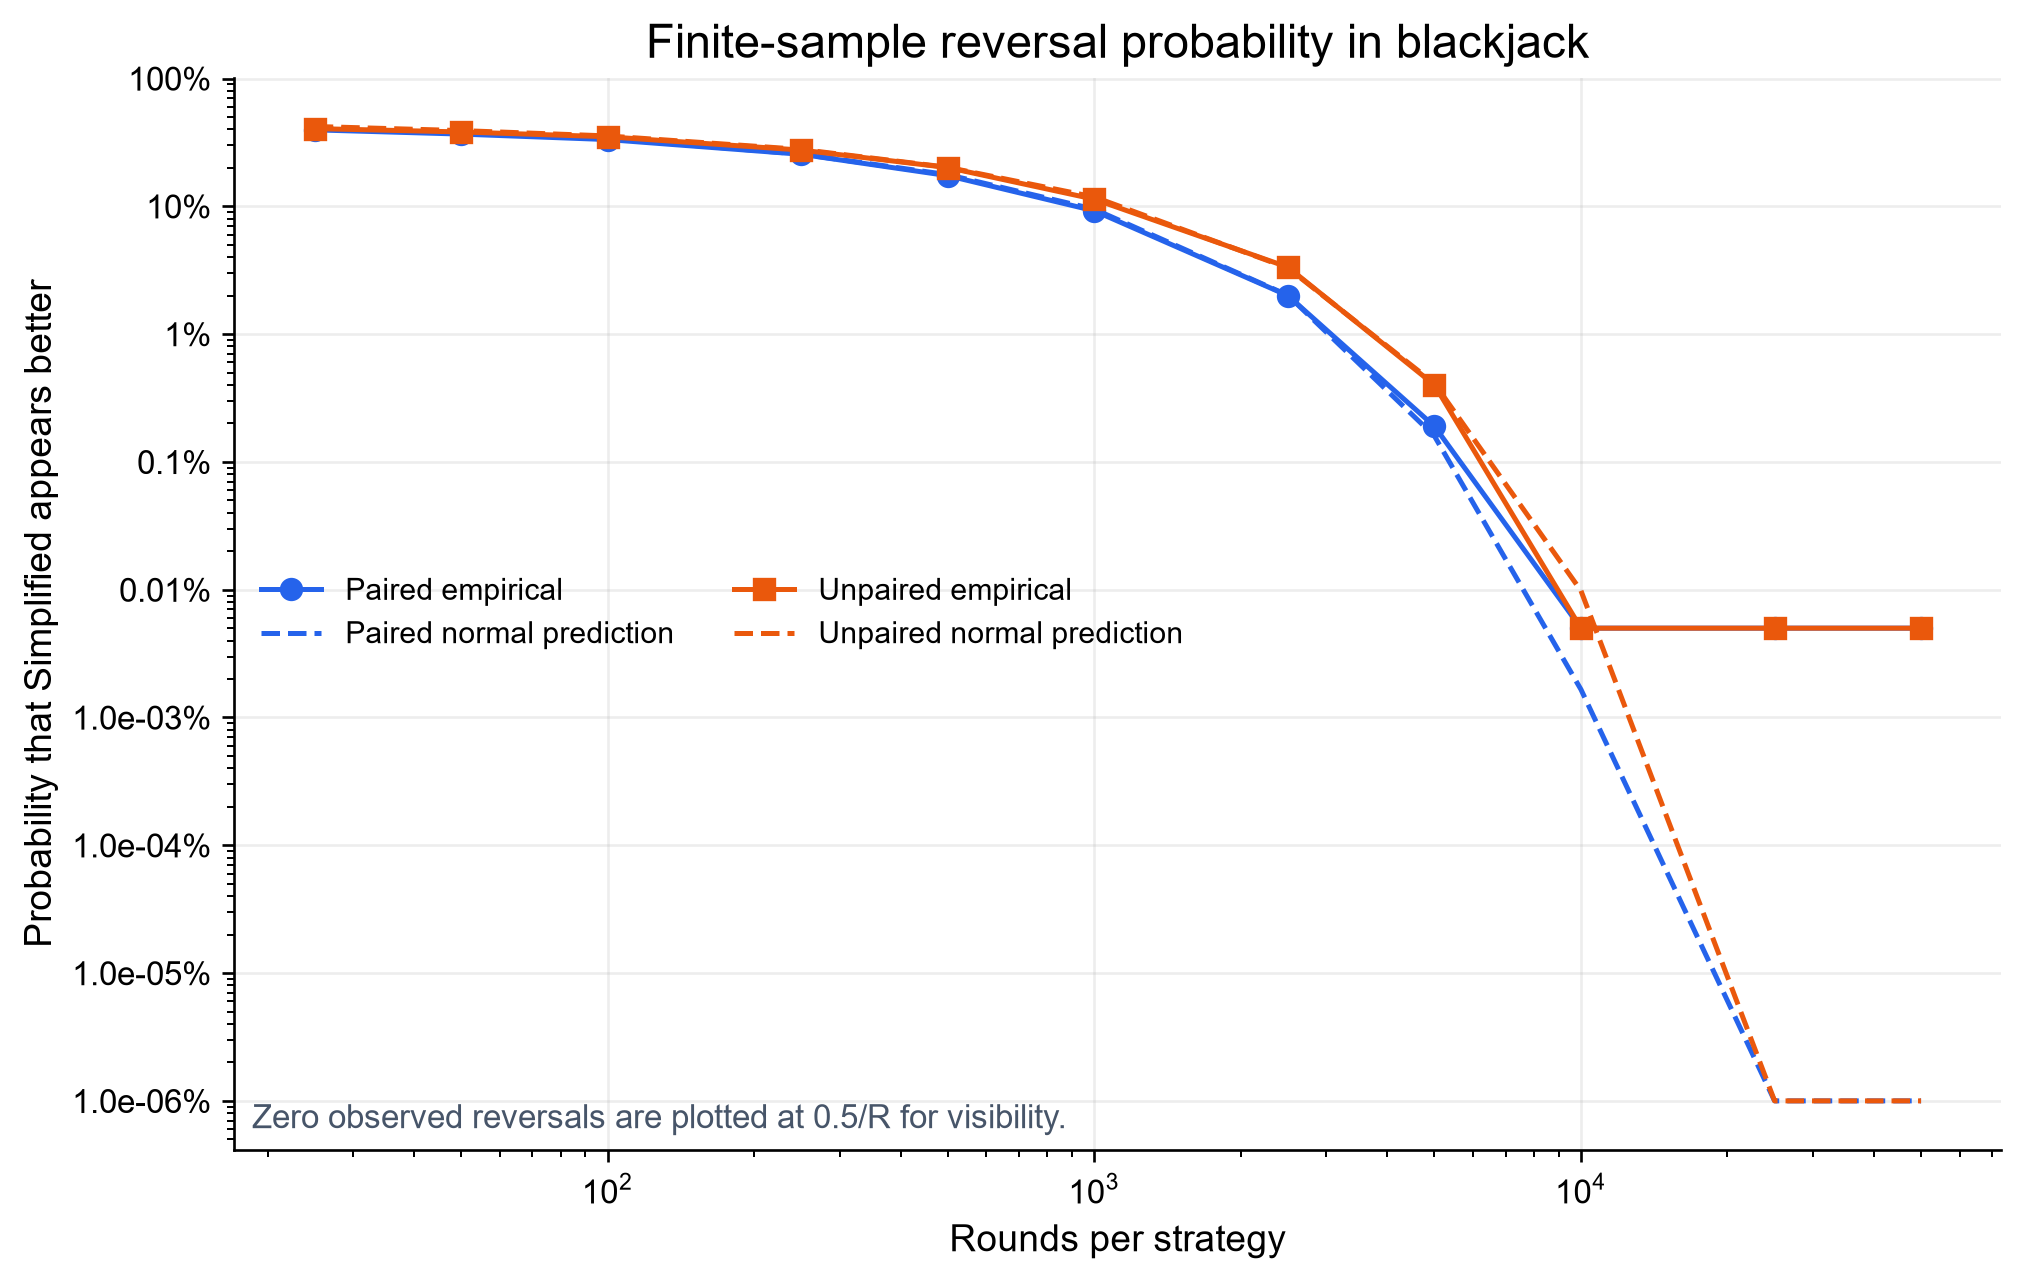
\includegraphics[width=0.90\textwidth]{../figures/01_blackjack_reversal_probability.png}
\caption{Empirical and normal-approximation blackjack reversal risk under
paired and unpaired evaluation.}
\label{fig:blackjack_reversal}
\end{figure}

\begin{table}[H]
\centering
\caption{Selected paired blackjack reversal probabilities.}
\begin{tabular}{rrrr}
\toprule
$n$ & Empirical & Normal & 95\% empirical interval \\
\midrule
100   & $33.29\%$ & $33.94\%$ & $[32.37\%,34.22\%]$ \\
500   & $17.37\%$ & $17.68\%$ & $[16.63\%,18.13\%]$ \\
1,000 & $ 9.22\%$ & $ 9.49\%$ & $[ 8.66\%, 9.80\%]$ \\
2,500 & $ 2.00\%$ & $ 2.01\%$ & $[ 1.73\%, 2.29\%]$ \\
5,000 & $ 0.19\%$ & $ 0.16\%$ & $[ 0.11\%, 0.30\%]$ \\
\bottomrule
\end{tabular}
\end{table}

\subsection{Pairing and Required Evidence}

Pairing reduced the variance of the blackjack strategy difference by a median
of approximately $19.6\%$. At $n=1{,}000$, reversal risk was $9.22\%$ under
pairing and $11.36\%$ under independent evaluation; at $n=2{,}500$, the
corresponding values were $2.00\%$ and $3.34\%$.

Using
\begin{equation}
n_\alpha=\left\lceil\left(\frac{z_{1-\alpha}\sigma_D}{\mu_D}\right)^2\right\rceil,
\end{equation}
the normal-planning sample requirements were
\begin{table}[H]
\centering
\caption{Blackjack sample-size requirements.}
\begin{tabular}{rrr}
\toprule
Target risk & Paired $n$ & Unpaired $n$ \\
\midrule
$10\%$  &   974 & 1,206 \\
$ 5\%$  & 1,604 & 1,987 \\
$ 1\%$  & 3,208 & 3,974 \\
$0.1\%$ & 5,660 & 7,012 \\
\bottomrule
\end{tabular}
\end{table}

At $n=2{,}500$, mean returns ranged from $-0.49\%$ for full basic strategy to
$-42.55\%$ for random legal play. The basic-strategy advantage over simplified
strategy remained positive under every tested rule variant. The largest rule
effect was the change from a $3{:}2$ to a $6{:}5$ blackjack payout.

Conditions through $n=2{,}500$ used direct finite-shoe simulation. Larger
conditions aggregated independently resampled matched 2,500-round blocks and
must not be interpreted as uninterrupted 50,000-round paths. Zero reversals
were observed in 10,000 replications for $n\geq10{,}000$, giving an exact 95\%
upper confidence bound of approximately $0.0369\%$, not proof of zero risk.

\newpage

\section{Inventory-Control Validation}

\subsection{Model and Analytical Optimum}

Let $D\sim\operatorname{Poisson}(20)$ and define
\begin{equation}
\pi(q,d)=12\min(q,d)-7q+2\max(q-d,0)-4\max(d-q,0).
\end{equation}
The underage and overage costs are $C_u=9$ and $C_o=5$, so the critical
fractile is $9/14=0.642857$. Since
\begin{equation}
F_D(20)=0.559093<\frac{9}{14}\leq F_D(21)=0.643698,
\end{equation}
the optimal integer order quantity is $q^*=21$. Moreover,
\begin{align}
\E[\pi(21,D)]&=76.298815, & \E[\pi(20,D)]&=75.126111,\\
\mu_\Delta&=\E[\pi(21,D)-\pi(20,D)]=1.172704.
\end{align}

\subsection{Pairing Through Common Demand}

Under common demand,
\begin{equation}
\Delta(d)=\pi(21,d)-\pi(20,d)=
\begin{cases}
-5,&d\leq20,\\
9,&d\geq21.
\end{cases}
\end{equation}
The exact moments are
\begin{align}
\operatorname{Var}(\pi_{21})&=647.7246,&
\operatorname{Var}(\pi_{20})&=491.3219,\\
\operatorname{Cov}(\pi_{21},\pi_{20})&=545.3655,&
\operatorname{Var}(\Delta)&=48.3156.
\end{align}
Independent evaluation has comparison variance $1139.0465$. Thus,
\begin{equation}
VR=1-\frac{48.3156}{1139.0465}=0.9576,
\end{equation}
so common-demand pairing removes approximately $95.8\%$ of comparison
variance.

\subsection{Exact Versus Normal Risk}

Let $p_h=P(D\geq21)=0.440907$. If $K\sim\operatorname{Binomial}(n,p_h)$,
then $\sum_i\Delta_i=14K-5n$, and the strict exact reversal probability is
\begin{equation}
P_{\mathrm{rev}}^{\mathrm{exact}}(n)
=P\!\left(K<\frac{5n}{14}\right).
\end{equation}

\begin{figure}[H]
\centering
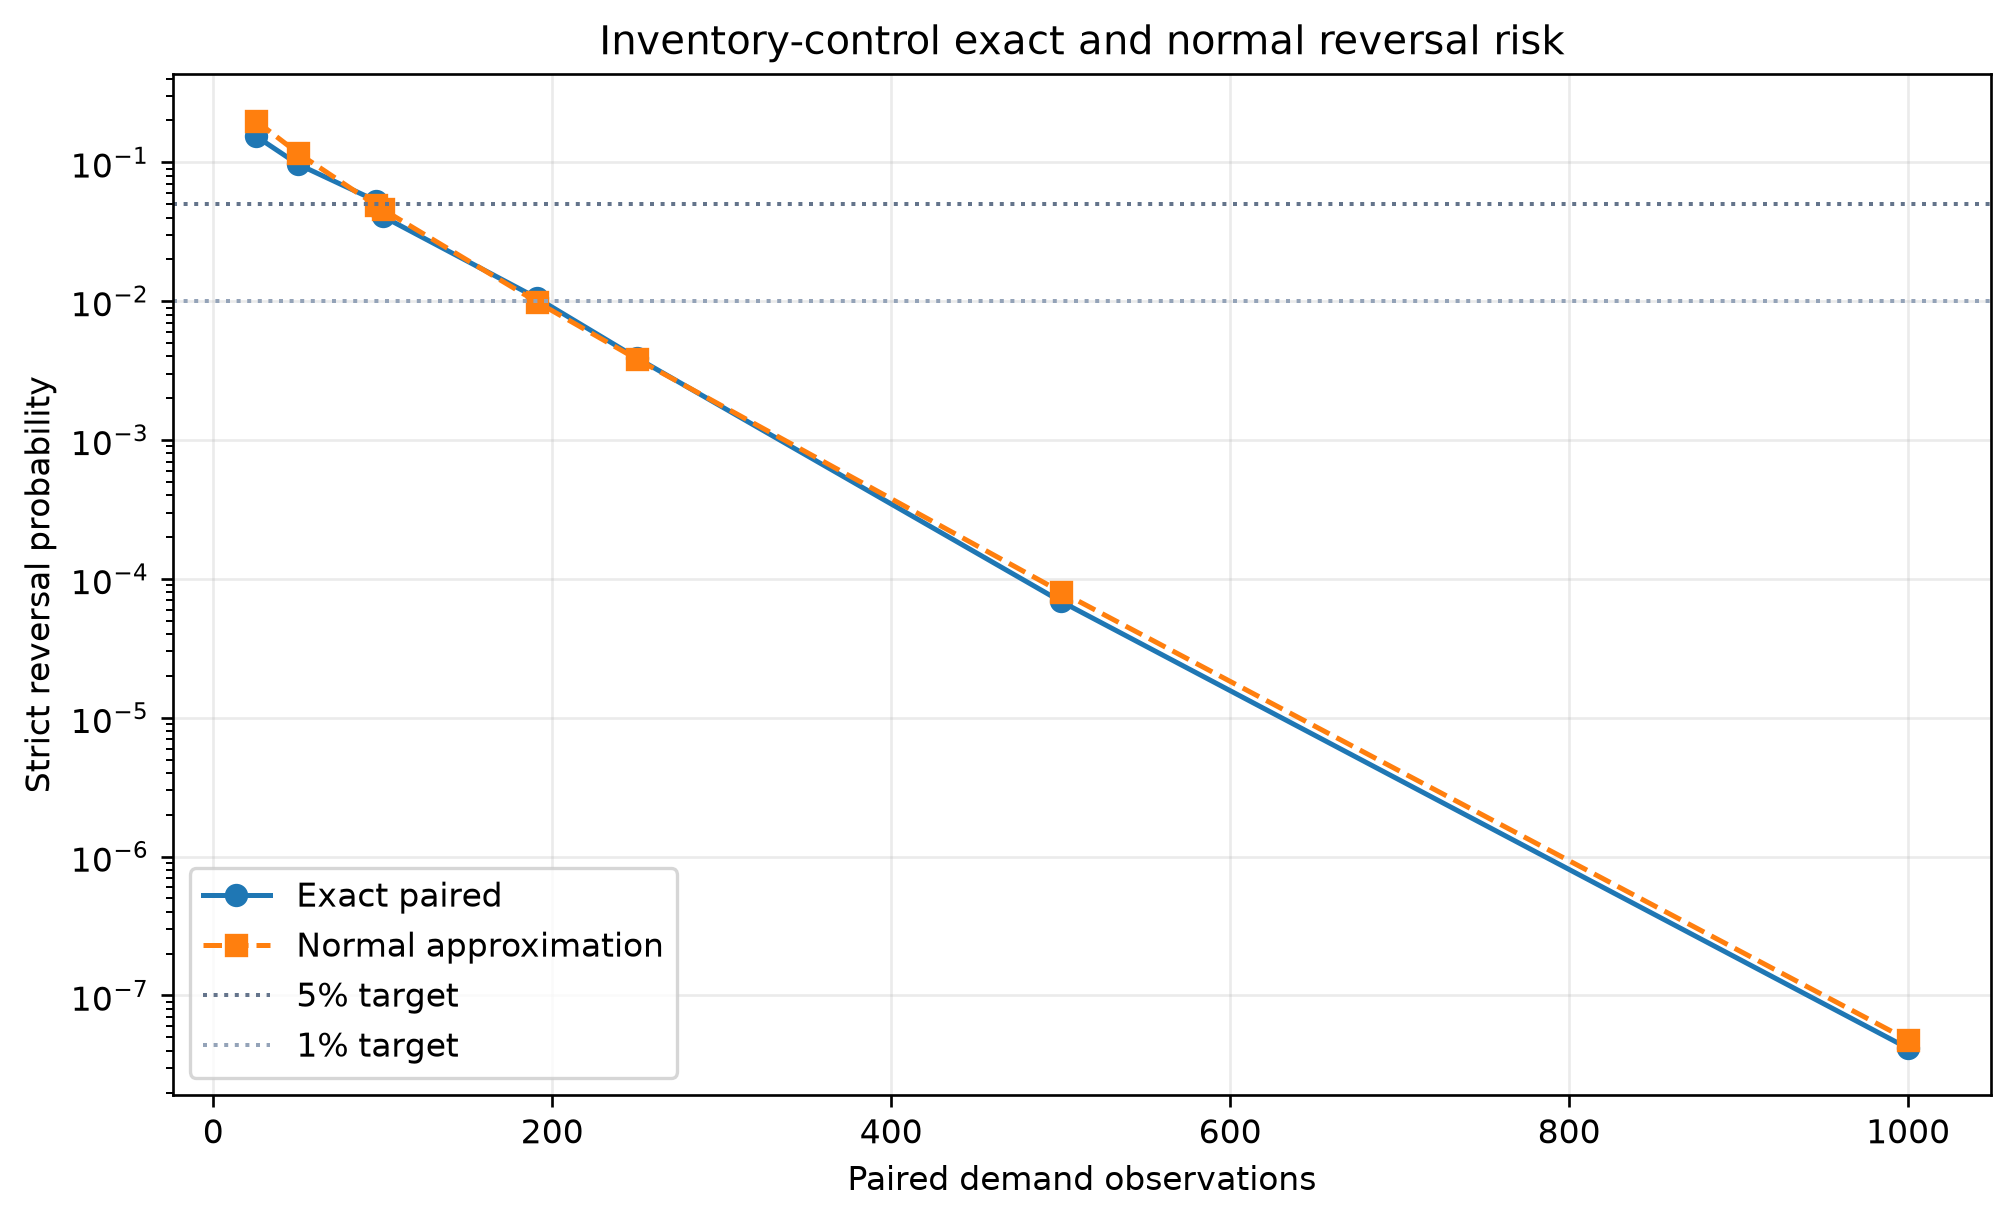
\includegraphics[width=0.90\textwidth]{../figures/11_inventory_exact_validation.png}
\caption{Exact and normal-approximation inventory reversal risk.}
\label{fig:inventory_exact}
\end{figure}

\begin{table}[H]
\centering
\caption{Normal planning and exact paired inventory risk.}
\begin{tabular}{rrrr}
\toprule
Target & Normal $n$ & Normal risk & Exact risk \\
\midrule
$5\%$ &  96 & $4.9163\%$ & $5.2844\%$ \\
$1\%$ & 191 & $0.9860\%$ & $1.0530\%$ \\
\bottomrule
\end{tabular}
\end{table}
Normal planning is therefore a useful approximation, not a finite-sample
guarantee. For comparison, the 5\% target requires approximately 2,241
unpaired observations but only 96 paired observations.

\newpage

\section{Controlled Bernoulli Exact Benchmark}

\subsection{Model Construction}

Let the environment be easy or hard with equal probability. Conditional on the
environment, $X$ and $Y$ are independent Bernoulli outcomes with
\begin{equation}
\begin{array}{c|cc}
 & \mathrm{easy} & \mathrm{hard}\\
\hline
P(X=1\mid E)&0.80&0.40\\
P(Y=1\mid E)&0.70&0.40
\end{array}
\end{equation}
so $\E[X]=0.60$, $\E[Y]=0.55$, and $\mu_D=0.05$.

\subsection{Exact Difference Distribution}

For $D_i=X_i-Y_i\in\{-1,0,+1\}$,
\begin{equation}
P(D_i=-1)=0.19,\qquad P(D_i=0)=0.57,\qquad P(D_i=+1)=0.24.
\end{equation}
Therefore, $\operatorname{Var}(D_i)=0.4275$. Independent evaluation has
variance $0.4875$, so pairing reduces variance by approximately $12.3\%$.

Let $(N_+,N_-,N_0)\sim\operatorname{Multinomial}(n;0.24,0.19,0.57)$.
Since $\sum_iD_i=N_+-N_-$, the strict exact reversal probability is
\begin{equation}
P_{\mathrm{rev}}^{\mathrm{exact}}(n)=
\sum_{\substack{a,b\geq0\\a+b\leq n\\a<b}}
\frac{n!}{a!b!(n-a-b)!}(0.24)^a(0.19)^b(0.57)^{n-a-b}.
\end{equation}

\begin{figure}[H]
\centering
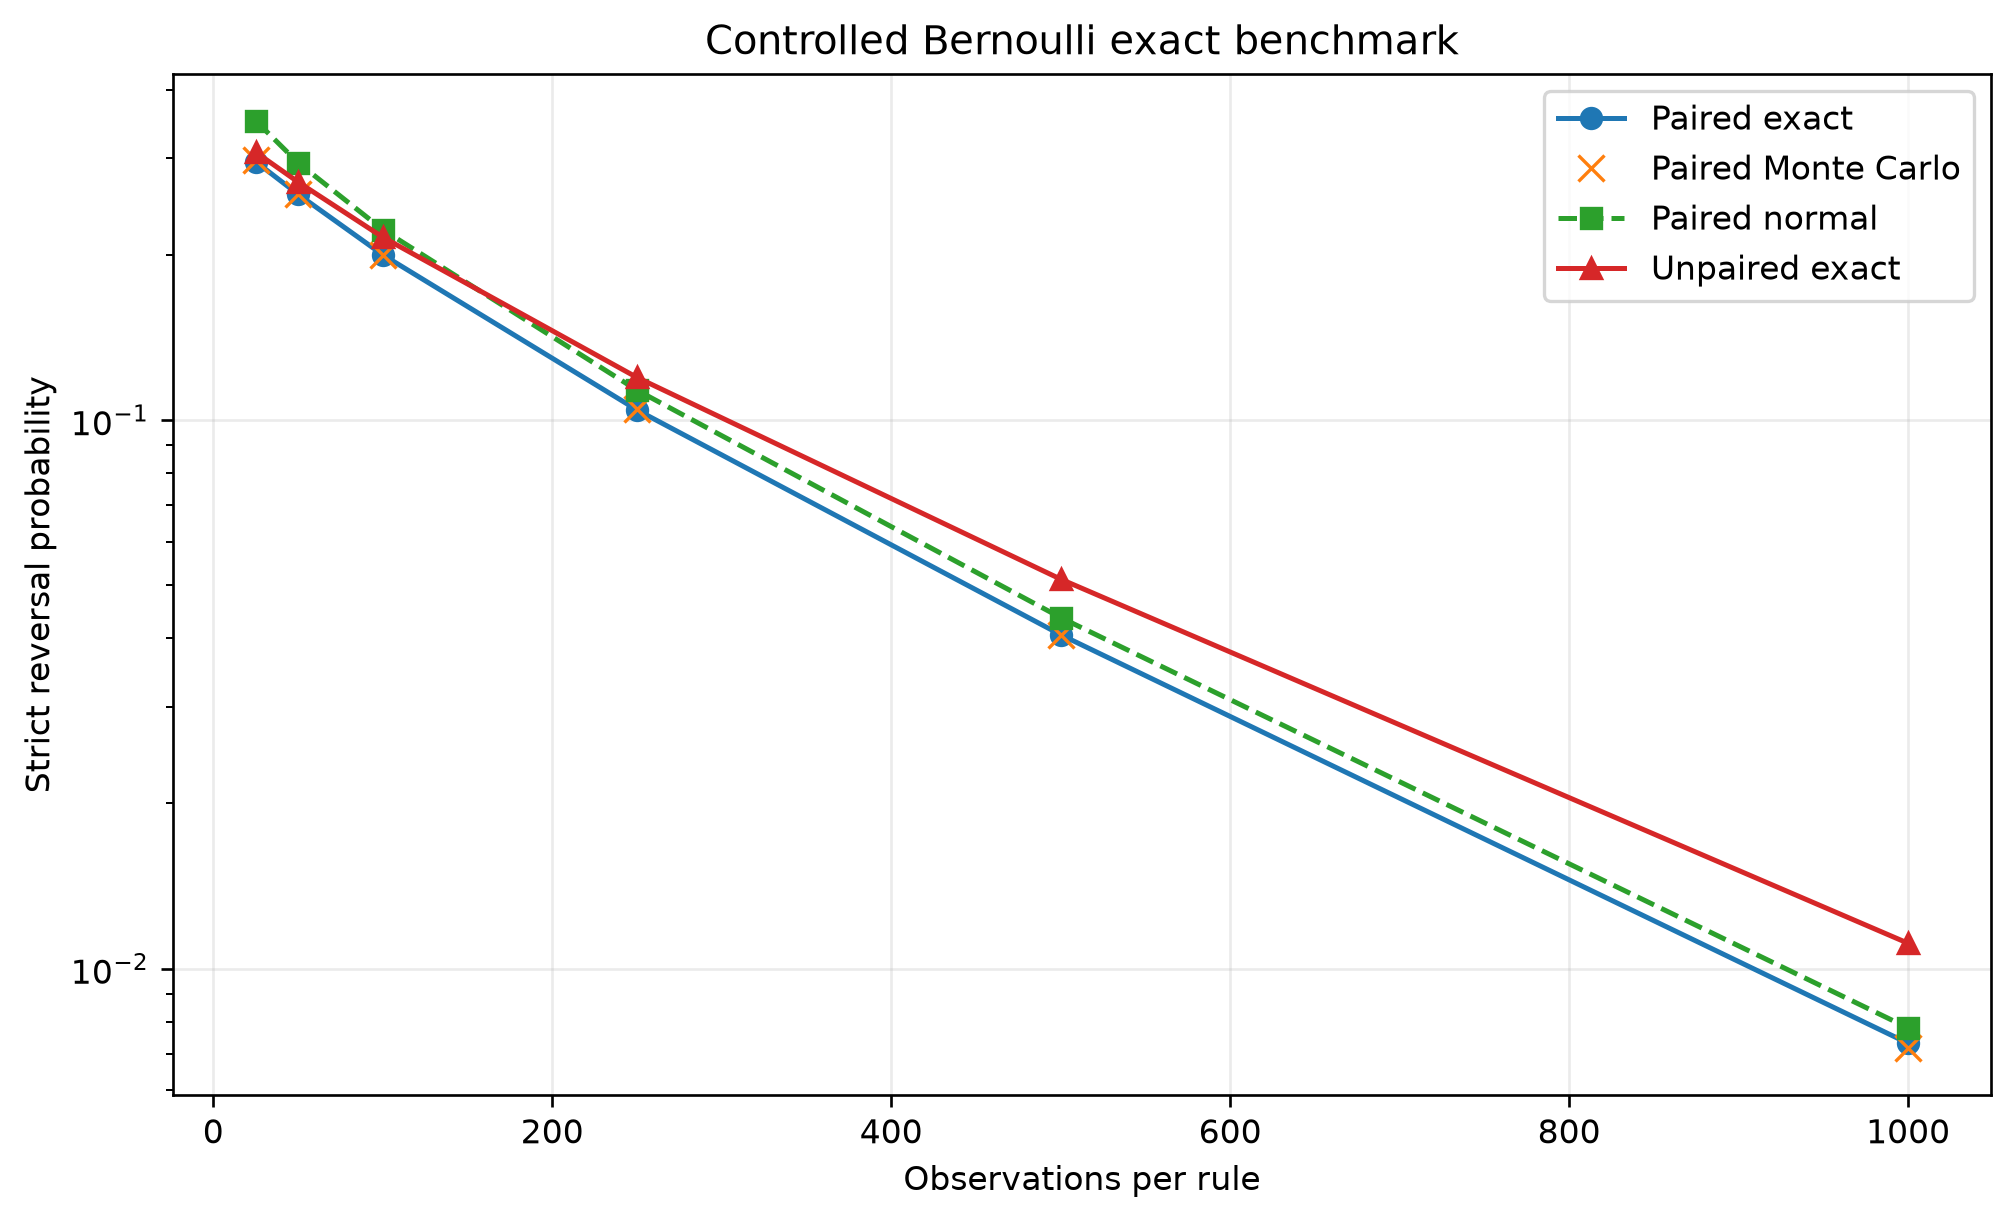
\includegraphics[width=0.90\textwidth]{../figures/12_bernoulli_exact.png}
\caption{Exact, Monte Carlo, and normal strict reversal risk in the controlled
Bernoulli benchmark.}
\label{fig:bernoulli_exact}
\end{figure}

\begin{table}[H]
\centering
\caption{Strict Bernoulli reversal risk. Monte Carlo uses 100,000 replications.}
\begin{tabular}{rrrrr}
\toprule
$n$ & Paired exact & Monte Carlo & Normal & Unpaired exact \\
\midrule
25    & $29.564\%$ & $29.778\%$ & $35.110\%$ & $30.766\%$ \\
50    & $25.787\%$ & $25.806\%$ & $29.434\%$ & $27.145\%$ \\
100   & $19.997\%$ & $19.939\%$ & $22.222\%$ & $21.532\%$ \\
250   & $10.429\%$ & $10.468\%$ & $11.331\%$ & $11.952\%$ \\
500   & $ 4.060\%$ & $ 4.055\%$ & $ 4.364\%$ & $ 5.127\%$ \\
1,000 & $ 0.731\%$ & $ 0.716\%$ & $ 0.780\%$ & $ 1.112\%$ \\
\bottomrule
\end{tabular}
\end{table}

The exact calculation separates strict reversals from ties. At $n=100$, for
example, strict reversal risk is $19.997\%$, tie probability is $4.548\%$, and
the combined nonpositive probability is $24.545\%$. Monte Carlo closely tracks
the exact benchmark, while the normal approximation improves as $n$ grows.
